\setcounter{figure}{0}
\setcounter{table}{0}
\setcounter{footnote}{0}

\articletitle{Use of Alternative Dispute Resolution methods for effective consumer protection- A Critical Analysis}\label{2017-art5}
\articleauthor{Sree Krishna Bharadwaj H\footnote{Research Scholar, National Law School of India University, Bengaluru}}
\lhead[\textit{\textsf{Sree Krishna Bharadwaj H}}]{}
\rhead[]{\textit{\textsf{Use of Alternative Dispute Resolution...}}}

\begin{multicols}{2}

\heading{Introduction:}

\noi
Dispute resolution has two prominent categories, namely Adversarial and Non-Adversarial i.e. Adjudicatory and Non-Adjudicatory. One of the most formal methods is Adversarial which includes trial and arbitration. This method, by virtue of being the most formalized methods, is also the most widely used methods of dispute resolution.\footnote{Rick Sarre, Alternative dispute resolution and non-adversarial regulation: why are they still not mainstream and can they ever become mainstream? Asia-Pacific Mediation Forum Conference, Adelaide, 29 November – 1 December 2001.} The Non-Adjudicatory methods of dispute resolution include Negotiation, Mediation, Conciliation, and Lok Adalat.

\heading{The differences between Adversarial and\\ Non-Adversarial process}

\noi
One of the most important differences between the two methods is that while the first method
involves a legally set up, due procedure and procedural laws, the latter does not involve any
due process.\footnote{Australian Law Reform Commission, Discussion Paper 62: Review of the Federal Civil Justice System. Sidney (1999).} The Non-Adversarial system is not coercive and the parties can withdraw
whenever they want.

\noi
The parties involved in a dispute have full control over the non-Adversarial system of dispute
resolution. In the Adversarial system, the focus is on facts and goes strictly by the facts
available on the table, whereas the non-Adversarial system considers relationships between the
disputing parties.

\noi
The Adversarial system looks at past and is regressive in nature. It goes by set precedents and
then arrives at a conclusion The Non-Adversarial system seeks to resolve issues in a manner
that maintains the goodwill relationship of the parties involved and keeps their future in
mind.\footnote{Judy Gutman, “The Reality of Non-Adversarial Justice: Principles and Practice”, 14 Deakin Law Review 29-51 (2009).} The Adversarial system establishes liability, whereas the non-Adversarial system focuses primarily on maintaining or in fact utilizing the relationship between the two parties.

\noi
The first method is thus a rather divisive method, whereas the latter is a more constructive
method aiming at arriving at rather amicable solutions for a given dispute.\footnote{ Harry N. Mazadoorian, “Putting together an ADR plan: The building blocks of a corporate program”, 3(1)
Business Law Today 40-44 (1993).}

\noi
As is visible with the judicial system, the Adversarialsystem establishes a clear-cut winner and
loser. The Adversarial system decides a winner and a loser involving lawyers and legal-experts
whereas the non-Adversarial system looks for a solution that is acceptable for all the parties
involved and the parties themselves play a crucial part in reaching a settlement.

\noi
Alternative Dispute Resolution solves issues in a cost-effective manner while preserving a
healthy relationship between the parties involved in the dispute.\footnote{Steven Shavell, “Alternative Dispute Resolution: An Economic Analysis”, 24(1) The Journal of Legal Studies1-28 (1995).} ADR tends to find different ways (beyond regular litigation) which can act as a suitable substitute for litigation and can resolve grievances and disputes, ADR is a procedure that is widely recommended in order to
reduce the number of cases by providing a cheaper, less adverse and economical type of justice
that is quite semi-formal and less complicated in nature. Even Judges recommend ADR to
reduce the number of court cases. The development of the information and the
communication technologies which are especially based on internet communications has
permitted the ADR services for moving into a whole new online virtual mechanism called
online dispute resolution.

\heading{Problems in Indian Judiciary}

\noi
Before understanding the problems of the judiciary, it is necessary to know some key concepts
which define some problems in the judiciary. Report No. 245 of the Law Commission of India
titled “Arrears and Backlog: Creating Additional Judicial (wo)manpower” gives the key
concepts as under:

\noi
Pendency: Case filed but have not been disposed of irrespective of when it was filed

\noi
Delay: When the adjudication takes more time than normal time for a similar case.

\noi
Arrears: Cases which are delayed more than the normal time but for valid reasons.

\noi
Backlog: If in a given time frame, the number of new cases filed is higher than the number of
cases disposed of, then the difference between the two is called backlog.

\noi
The Report also gives the increasing pendency of cases in the judiciary. It is to be noted that
the pendency of cases is on a rise in the higher judiciary while the disposal rate is constant in
the lower judiciary.
\end{multicols}

\vspace{-.4cm}

\begin{figure}
\centering
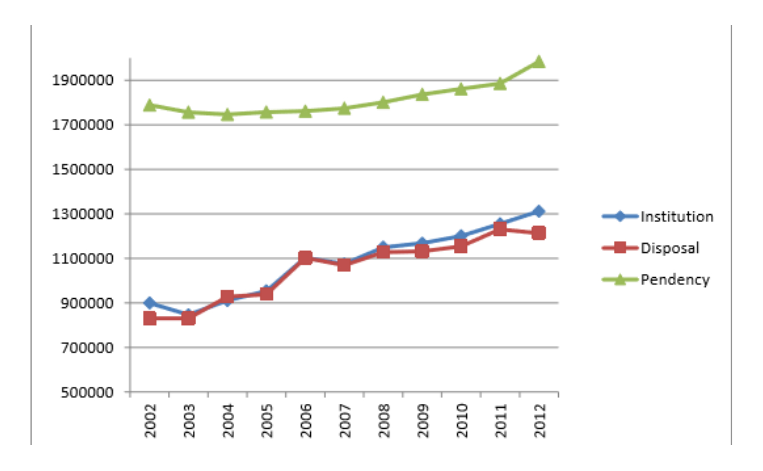
\includegraphics[scale=.85]{src/images/chap5/001.eps}
\caption*{\textbf{Graph 1: Cases filed, Disposed, Pendent in the “Higher Judicial Service” during 2002-
2012.}}\label{fig01}
\end{figure}

\vspace{-.4cm}

\begin{figure}
\centering
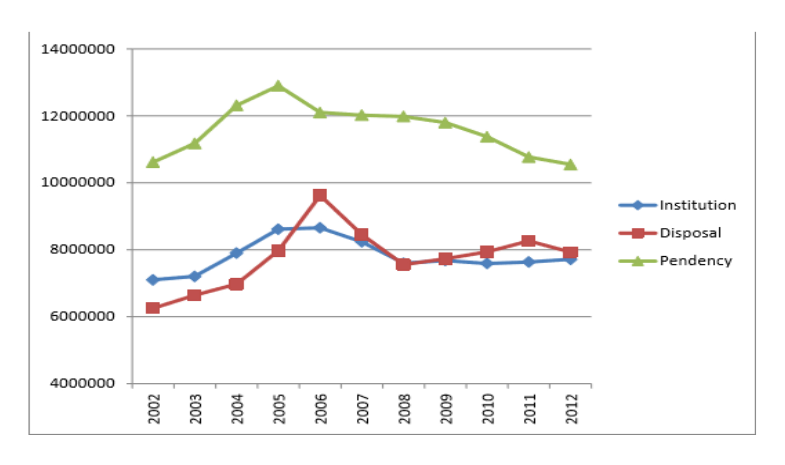
\includegraphics[scale=.85]{src/images/chap5/002.eps}
\caption*{\textbf{Graph 2: Cases filed, Disposed, Pendent in the “Subordinate Judicial Service” during
2002-2012.}}\label{fig02}
\end{figure}

\newpage

\begin{figure}
\centering
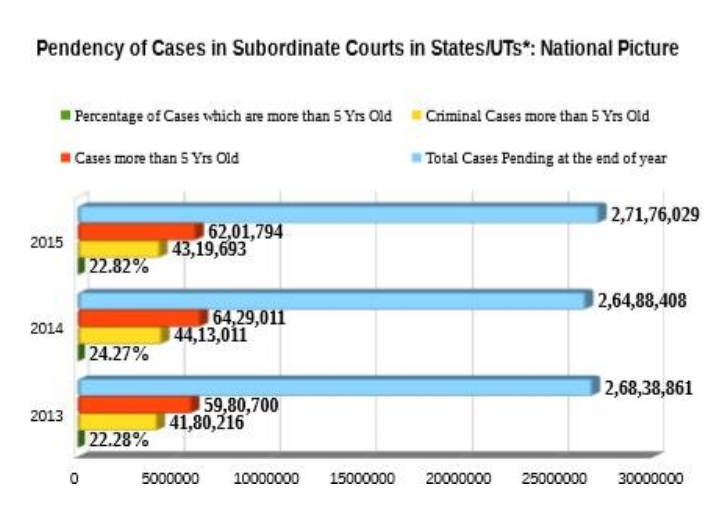
\includegraphics[scale=1]{src/images/chap5/003.eps}
\caption*{\textbf{Graph 3: Cases’ pendency in the “Subordinate Courtsin States/UTs” during 2013 to 2015}}\label{fig03}
\end{figure}

\vspace{-.5cm}

\begin{multicols}{2}
\vspace{-.3cm}
\noi
A report by Centre for Research \& Planning, Supreme Court of India, New Delhi titled
“Subordinate Courts of India: A Report on Access to Justice 2016” highlights the problems of
judiciary with respect to pendency and vacancies as under:
\end{multicols}

\vspace{-.2cm}

\noi
{\fontsize{8}{10}\selectfont
\begin{tabular}{|c|c|c|c|c|c|c|c|c|c|}
\hline
{\bf Year} & {\bf Opening}  &{\bf Institution} & {\bf Disposal} & {\bf Pendency} & {\bf Cases more}   & {\bf Criminal Cases}  & {\bf Sanctioned}  &{\bf  Working}& {\bf Vacancy}\\
     & {\bf Balance}  &            &           &          & {\bf than 5}   & {\bf more than}     &{\bf Strength} & {\bf Strength} & \\
     &           &          &           &           & {\bf Yrs Old} &  {\bf 5 Yrs Old}                  &                 &          & \\ \hline
2015 & 2,65,09,688 & 1,90,44,877&1,83,78,256&2,71,76,029&62,01,794&43,19,693&20,558&16,176,&4,382\\\hline 
2014 & 2,68,39,293&1,92,81,971&1,93,28,283&2,64,88,408&64,29,011&44,13,011&20,174&15,585&4,589\\\hline
2013&2,69,07,252&1,8670,907&1,87,37,745&2,68,38,861&59,80,700&41,80,216&19,526&15,128&4,398\\\hline           
\end{tabular}}

\begin{multicols}{2}

\noi
The Supreme Court and High Courts have realized that the task of clearing all the pending cases
by the judiciary is next to impossible. They also suggest the use of ADR methods for clearing
of the pendency of cases. The Legal Services Authority was set up with the purpose “to
organize \textit{Lok Adalats} to secure that the operation of the legal system promotes justice on abasis
of equal opportunity.”\footnote{Preamble to the Legal Services Authority, 1987.} Supreme Court has released mediation training manual\footnote{The same is \textit{available at:}\\ \url{http://supremecourtofindia.nic.in/sites/default/files/Mediation}\%20Training\%20Manual\%20of\%20\\India.pdf} and various High Courts have framed the Rules for court-annexed mediations. ADR is now being considered as an essential element of the justice system by both the legislature and the judiciary in the country. The National Consumer Dispute Redressal Commission also has permitted the use of ADR for dispute resolution at consumer fora level.\footnote{Bijoy Sinha Roy by Lr. vs Biswanath Das, 2017 (11) SCALE 391}

%~ \vspace{-.2cm}
\newpage
\heading{Effectiveness of CPA, 1986}

\vspace{-.2cm}

\noi
Evaluation Report on Impact and Effectiveness of Consumer Protection Act, 1986\footnote{Indian Institute of Public Administration (IIPA), Evaluation Report on Impact and Effectiveness of Consumer  Protection Act, 1986, (2013), available at: \url{http://www.consumereducation.in/ResearchStudyReports/cpa_exec_sum.pdf} (visited on: January 21, 2016).}

\noi
The impact of the Consumer Protection Act can be found with some statistical data retrieved
from the research. The data says that, about 43.7 percent of the consumers who have gone
through exploitation have stayed idle without filing complaint or any necessary action. This
might be due to various reasons like financial inability of the exploited consumer, fear of the
opponent, time issues and other unidentifiable reasons. In the end, all of them have just set the
problem aside with no concern. The next case is quite similar to the first one but has got a
difference in approach. About 41.7 percent of consumers have not taken the matter legally or
just left it unnoticed. Instead, they have made a try to get the price of the defective product
refunded. This category not only denotes price return, but also the replacement of the whole
product. And 17.3 percent have tried to mobilise the issue. Out of 100, only four percent of the
consumers have made complaints to the manufacturers and the producers of goods. Rest ninetyfour percent were left ignored or did not complain even in the district forum. All these problems
have a central reason, which is nothing but poor awareness about the act and the process. On
seeing the knowledge or awareness level that has reached the public, 67.2 percent of the
exploited consumers are unaware ofthe fact that there is something called Consumer Protection
Act. Some know about the Act in depth and their percent is 10.2. The rest comprising of 22.6
percent have minimal knowledge about the Act and the redressal techniques available for
affected consumers. The data retrieved has clear information with regards to even gender and
age. In gender perspective, unawareness is seen in about 63.5 percent in male category, and 71
percent in female category. And with the view of age, 70.2 percent of people below the age of
thirty are unaware of the Act and the 61 percent of people who fall above the age of fifty are
with no knowledge about the Consumer Protection Act. These percent values are to make clear
views on the present condition of the Act and to notify that more awareness is needed.

\noi
The first reason was that there were adjournments made without actual necessity at that place.
As already mentioned, the cases and complaints made cannot be adjourned as and when
required without any reason under the grounds of a “sufficient cause”. Also, the reason for
these adjournments should be made as written record for later evidences. It accountsfor twenty-seven percent ofthe whole reasons for the delay. The next reason would be poor administration.
Poor administration here means the less skilled staff or inadequate number of workers in the
commission for carrying out the whole process. Also, there should be an efficient
administrative control within the commission to follow up the case and to make sure that all
the cases admitted are brought for proceeding. Cases can at times be recorded as a disposed
case even before the proceeding. Such errors occurred are purely due to improper
administration. Support staffs are an integral part of any working body and when it comes to
commissions handling consumer disputes, it is mandatory to have a very decent strength of
support staff. There should not be work stoppage due to less support staff since it might
interrupt a very expensive process. Apart from this proper administration is very necessary to
maintain the infrastructure of the office as they may reveal the very first impression of the
performance of the office. This reason amounts to about nineteen percent of the total reasons
causing late disposal of cases. The last reason is bound to the consumer’s nature or is a
consumer’s inherent disadvantage. Exploitation happens if the person harmed is uneducated.
Not that educated people do not fall under the umbrella of exploitation, but the chances are
high when it is about illiterates. It gives the confidence to the sellers or providers of a defective
product or deficient service that the victim will not take further steps to file a case on him.
There arise the problems for the uneducated victims. Now, this illiteracy or poor education
stands as a reason for the delay in disposal of cases too. The victims who file case on the seller
or provider basically suffers from the inability to survive the whole process without proper
knowledge.

\noi
Legal documentation or any work requiring education will be a barrier to these victims and it
finally prolongs the case. Hence, poor education will also be taken as a reason if there is a delay
in the case disposal and this reason takes eleven percent share of the total reasons. Vacant
positions of the President and Members of the commission takes a huge part in interrupting the
services of the commissions. It is a known fact that if there are no appointed people in the
respective posts, their responsibility will be left unnoticed or undone. The fact has proven in
this case, and there has been a tremendous delay in disposal of cases due to vacancy of
positions. The next reason is the limited or very less number of benches of the commissions.
Restricted infrastructure and very less space may also be an issue for operation of any
organisation. Similarly, poor infrastructure has created an impact on the cases involved and has
created a situation of late disposal of cases. Insufficiency in the required tools to execute an
operation is also a drawback of the infrastructure which leads to uncleared cases. Some cases 
will demand for a clear investigation or analysis to arrive at a decision. In such a situation, there
exists excess time duration of the investigation process resulting in the breakdown of thewhole
system even if one of the processes stop working or is held for any valid reason. Test reports
are very important to provide a fair judgement or to make further move in a case. If there is a
considerable delay in receiving the reports, there will definitely be delay in the processof clearing
the case. The case might be held uncleared if the test reports completely don’t reachthe
commission even after providing excess time. Starting from a basic business firm to the
court/forum, training for every individual working is mandatory. Training and learning together
is a process which should be indulged in all the organisations to preserve the rules and
regulations set in it. Ifthere is a member or a president in a commission without proper training,
the duties allotted for them will not be efficient in the output. They will lag more in terms of
quality and time while performing an operation of the commission. This condition also takes
the case handled to a state of uncleared case or delayed disposal. Redressal may be slow even
due to insufficient funds from the consumer’s side. The complainant who has filed a case
should be ready with the necessary finance to travel through the whole process without any
interruption. The cases taken might not be redressed at its earliest if the complainant fails to
make any required payment during the process. Thus, the financial status of the complainant is
also an important factor to be taken into consideration to make sure that there is no delay in
redressal. All these reasons are provided in values of percentage to show each reason’s share
in the total percent. They are as follows,

\vspace{-.4cm}

\begin{enumerate}[label=$\bullet$]
\itemsep=0pt
\item Vacancy of positions – nine percent

\item Limited number of benches – eight percent

\item Poor infrastructure - seven percent

\item Delay in lab testing - five percent

\item Insufficient training - four percent

\item Complainant’s ability to pay – three percent
\end{enumerate}

\vspace{-.4cm}

\noi
Minor reasons which amount to delay in redressal

\vspace{-.4cm}

\begin{enumerate}[label=$\bullet$]
\itemsep=0pt
\item The summons and notices sent by the commissions may not reach the consumer or the
complainant on time and here starts the issue of delay. The person receives it late, then
responds late and finally the whole process becomes more time consuming making the
redressal lingering. This delay in the receiving of the summons and notices is due to the
channel by which they are sent. Postal couriers are the only means by which these
notices are sent and fault from courier’s side cannot be accounted for the delay in
redressal or late delivery of the notices.

\item Accumulation of uncleared or undisposed cases makes the commission unable to handle
the newly admitted cases. A number of the case pending in the commission demands
for redressal making the new cases delayed. And it goes as a cycle where thecourt or
commission finally makes an increase in the pendency of cases.

\item Funds for operation and carrying out the necessary processes in the commissions and
forums are not available always. This poor financial status holds the process as and
when there is a necessity. Thus, the source of money is a problem which makes the
commissions unable to work.

\item While appointing a judicial member, the qualifications needed are checked for but the
training aspect is missed out. The member appointed in the commission holds only the
qualification for the position and is unaware of the practices and customs of the
commission. Training is thus a very important factor which decides the functioning of
the commission and if it is a drawback, then the cases handled will be delayed in
redressal.

\item Another rare reason for the delay in redressal would be the illegal strikes happening
around the state. Due to these unavoidable or undesirable happenings, the commission
has to stop function for two or three days till the strike is closed. Meanwhile, the cases
stay pending or will be redressed with the delay in future.

\item Employee satisfaction is a catalyst for better output by an organization. The members
of the commission should be given appropriate amounts ofsalary and incentives as and
when there is a need. This is the only motivation which will lead to increased level of
performance. But, unfortunately, the commissions have lost in this aspect by giving less
salary to the members. Also, the transport facilities demanded by the members were not made by the commission. All these issues have led to delay in redressal making it clear
that poor compensation will end up in poor performance.

\item There is one more situation where the case after passing the order, will stay uncleared.
This is because the judgment made needs the approval of the district collector or the
police department of the respective location. Hence, the implementation of the orders
is becoming complex due to approval by various office bearers. If there is
implementation of the commission, the number of cases pending will reduce to a great
extent.
\end{enumerate}

\vspace{-.5cm}

\noi
Members who feel that there is an efficient operation in the commission fall were 24 percent
and the rest still have not realised or felt the empowerment in the functioning of the
commission. They found few reasons for such a situation with close supervision and efficient
analysis. The first reason was a very common one which pointed the delay in redressal. No
matter how efficient a system is, if the factor called timeliness is lost the whole system stands
unfit or non-productive. Having said this, the commissions should take measures in order to
reduce the time taken for each case. The orders passed should be implemented/executed within
the commission and its absence makes the members feel that the commission holds less power.
The authority to pass orders after every case should be given to the commission which will
indirectly create a positive impact on the time taken for the redressal of cases. Strict rules should
be made regarding adjournments where the case cannot be adjourned according to the party’s
wish. No case can be adjourned without stating explicit and valid reason inwriting. Themembers
feel that the commission suffers from this control of adjournments and have stated that this is
also a reason for inefficiency of the commission. The members have pointed the reason for the
low efficiency of the commission as poor empowerment status of the commission when
compared to the empowerment status of the civil courts. They feel that the rights and powers
of the civil court is far more than the commission because of which the commission isquite not
chosen as the best option to deal with cases. Also, on the part of compensation provided to the
consumers or the plaintiff, the commission orders only a very less amount. Recovery and refund
do not completely compensate the loss faced by the complainant. This reason completely
eliminates the commission from being called as an empowered one.


\heading{State of the Indian Consumer 2012\footnote{Consumer Unity \& Trust Society (CUTS International), State of The Indian Consumer Analyses of the Implementation of the United Nations Guidelines for Consumer Protection, 1985 in India (2012), available at: \url{http://www.cuts-international.org/Cart/pdf/State_of_the_Indian_-Consumer.pdf} (visited on: January 12, 2016).}}

\noi
Though the exploited consumers or the complainants can represent themselves in the
commissions, only a few consumers do so and the rest finds a substitute for it. The consumers
are mostly represented by the advocates in the State Consumer Dispute Redressal Commission
and the District Consumer Dispute Forum. Other few will represent themselves by nonGovernmental organizations or by the government. They are as follows,

\vspace{-.3cm}

\begin{enumerate}[label=$\bullet$]
\itemsep=0pt
\item Self - representation -nine percent

\item Representation by commissions and forums – eighty-nine percent

\item Representation by government bodies and non-governmental organizations – one percent each
\end{enumerate}

\vspace{-.3cm}

\noi
The summary of the survey

\vspace{-.3cm}

\begin{enumerate}[label=$\bullet$]
\itemsep=0pt
\item The summary has come up with few findings relating to the commission and the
behavior of the consumers.

\item About three-fifths of the exploited consumers do not take the issue to the commission
or civil court, instead, they deal it directly with the sellers or the last person of the
supply chain from whom the product was purchased. Complaints are made directly to
the seller without involving any legal body to address the issue.

\item There is another group of consumers who have not taken any action for the loss they
have faced. They have neither complained to the seller nor made the case to be
addressed by the commission. This group accountsfor about ninety-three percent of the
whole exploited consumers. Another group of consumers accounts for three percent
who have registered the complaint with the product’s company. In the end, the survey
reveals that only 0.3 percent of the affected consumers have really approached the
consumer for a seeking redressal. This means that the efficiency and the existence of
the consumer for a should be well communicated. More awareness programmes should be created in all possible areas for creating knowledge about these commissions in the
minds of people. Also, the techniques of redressal should be informed so that a sense
of trust arises and with that, they approach the commission for redressal.

\item In the survey, about four-fifths of the respondents have marked that the process of
redressal through these commissions as tedious. On seeing the reasons for such an
answer, it is seen that the commissions have failed to make the process clear and
simpler. The complexity of it has stopped many of the consumers from approaching the
commissions for redressal. Also, three-fourths of the admitted cases were not resolved
as desired. There were confusions and commotions with the case disposal. And among
this, eighteen percent of the undisposed cases were handled by the higher authorities
for redressal as an appeal. This change means that the lower authorities are quite
inefficient in handling the case.

\item Poor timing maintained for case disposal was also a finding of the survey. About twothirds of the cases were not solved or provided with a judgment in a given time frame.
Most of the cases were pending and it took a very long time to even initiate the case
again. The survey says that the cases take more than the fixed time of 100 or 150 days
to get solved. There are situations where few cases are left pending even for more than
ten years. Adjournment, poor number ofsupport staff and the illiteracy condition of the
complainants may be the three reasons contributing for the delay in disposal of cases.

\item On the fifth of the respondents marked a mistake in terms of money. They have felt that
the method of redressal demand for more money. This expensive process thus stays
inefficient due to direct coststhat have to be paid by the consumes or the complainants.

\item Also, there is unawareness about the inherent redressal mechanism provided by the
company. This unawareness is seen in about fifty-five percent of the consumers.

\item Seven percent of the consumers have a strong belief that the inherent redressal
mechanism in the companies does not facilitate transparency in handling the issues.
There is suspicion about the reliability of the company too.

\item And there is one more crowd which does not even know that there is redressal
mechanism outside the company. These people amount to about fifty-three percent and
are more towardsthe redressal mechanism provided internally.

\item Regarding the accessibility, the respondents have made points stating that the redressal
mechanism cannot be accessed by a common man since those mechanisms are highly
independent. Also, few others have stated that it is possible to access it easily. They are
separated as thirty-eight percent in the first category and twenty-seven percent in the
next category.

\item A sense of trust is created only in twelve percent of consumers. This group strongly
believes that the functioning of these redressal mechanisms is very positive and will be
a one favoring the consumers. They also believe that the capability of redressing the
issues and the level of security here in these redressal systems is high.

\item From the consumer forum about thirty-four percent of people believe that consumer
education will be helpful in making the redressal process a very smooth one. Also, the
rights that can be availed by the consumers should be informed to them so that they
know how to handle various issues. Another group of members holding twenty-four
percent, opine that the consumers can be provided with legal and technical assistance
to make the process more convenient.

\item Finally, only twenty-four percent of the State Consumer Dispute Redressal
Commission has accepted that they are sufficiently powered to try all cases. Rest of
them are still in the status of a dilemma to decide on the efficiency of the commission.
\end{enumerate}

\vspace{-.3cm}

\noi
Thus, it is clear from the above that neither the mainstream judiciary nor the quasi judicial
structure under the Consumer Protection Act, 1986 are good for the consumers who want swift
justice which is inexpensive as well.

\heading{Importance of Alternative Dispute Resolution}

\noi
Alternative Dispute Resolution is regarded as a grievance solving system outside the doors of
the court of the country. Alternative Dispute Resolution mechanisms give the parties the
freedom and flexibility to solve disputes with harmony and with ease instead of taking it to the court for claim via the formal procedure of the court.\footnote{Faye A. Silas, “Settling disputes: Law firms get into ADR act”, 72(4) ABA Journal 37 (1986).} Alternative Dispute Resolution is now
an important part of the civil judicial system of the country and has developed on its own
way.\footnote{Anurag K. Agarwal, “Resolving Business Disputes Speedily”, 41 (21) Economic and Political Weekly 2417- 2418 (2006).} ADR is the result when the search is of a simple, fast and flexible dispute solving system.
The main objective of ADR is to avoid vexation, high expenses and time consumption in
decision making which has made it the ideal form of seeking Justice, the Alternative Dispute
Resolution techniques are conciliation, arbitration, mediation, hybrid procedures, and
negotiations. Parties can exit the ADR methods when they wish and all methods in the ADR
methods are voluntarily reached.\footnote{Robert D. Raven, “ADR: New Options for Clients” 75(6) ABA Journal 8 (1989).}

\heading{ADR in other laws}

\noi
ADR methods have been extensively used in laws. Some of these are mentioned below:

\vspace{-.2cm}

\begin{enumerate}
\itemsep=0pt
\item Industrial Disputes Act, 1947: Section 2(p) of the Act defines Settlement as – “(p)
settlement" means “a settlement arrived at in the course of conciliation proceeding and
includes a written agreement between the employer and workmen arrived at otherwise than in
the course of conciliation proceeding where such agreement has been signed by the parties
thereto in such manner as may be prescribed and a copy thereof has been sent to an officer
authorized in this behalf by the appropriate government and the conciliation officer;”

\noi
The Conciliation officers are given the duty of mediating and resolving the disputes amicably
as given under Section 4(1).

\noi
“(1) The appropriate government may, by notification in the Official Gazette, appoint such
number of persons, as it thinks fit to be conciliation officers, charged with the duty of mediating
in and promoting the settlement of industrial disputes.”

\item The Hindu Marriage Act, 1955: The provision provides that the court shall give due
consideration towards the counseling and reconciliation of the parties.

\noi
“Before proceeding to grant any relief under this Act, it shall be the duty of the court in the first
instance, in every case where it is possible so to do consistently with the nature and circumstances of the case, to make every endeavour to bring about a reconciliation between the parties.”\footnote{Section 23(2)}

\item The Family Courts Act, 1984: Section 9 of the Family Courts Act says that wherever possible the Family Court shall try to settle the matter.\footnote{Section 9}

\noi
“In every suit or proceeding, endeavour shall be made by the Family Court in the first instance,
where it is possible to do so consistent with the nature and circumstances of the case, to assist
and persuade the parties in arriving at a settlement in respect of the subject-matter of the suit
or proceeding and for this purpose a Family Court may, subject to any rules made by the High
Court, follow such procedure as it may deem fit.
\end{enumerate}

\vspace{-.4cm}

\noi
If in any suit or proceeding, at anystage, it appearsto the Family Court that there is a reasonable
possibility of a settlement between the parties, the Family Court may adjourn the proceedings
for such period as it thinks fit to enable attempts to be made to effect such a settlement.”

\vspace{-.1cm}

\noi
It may also be noted that while Section 89, CPC confers the jurisdiction on the court to refer a
particular dispute under its consideration to an ADR mechanism, it is Rules 1A, 1C of Order
X that lay down the manner in which the court is supposed to exercise its jurisdiction. It may
be noted that the number of options available for availing ADR path, permit the parties to
choose the process by consensus. If the consensus is not reached, the mechanism allows
resuming of the legal process.

\vspace{-.1cm}

\heading{Mediation under Consumer Protection Bill, 2015}

\vspace{-.2cm}

\noi
As discussed in the previous chapter, the Consumer Protection Bill contains a separate chapter
on Mediation. The process of mediation is briefly explained below.\footnote{Chapter V of the Bill}

\noi
After the admission of a complaint in the district forum, if there is any sign present in the
complaint showing the possibility of redressing it through mediation, then the commission can
direct the case to the mediation process. However, this cannot be done in cases where there are
loss or serious conditions of injury or death to the consumer. The cases can be directed for
mediation after one hearing or at any stage during the proceeding.

\noi
There should be proper guidance given by the district forum regarding the processes of
mediation. Also, the decision of the consumers to opt for mediation is to be considered before
directing them to such a settlement.

\vspace{.1cm}

\noi
After arriving at a decision to solve the dispute through mediation, it is mandatory for the
parties to submit an application to the commission regarding the use of mediation for redressal.
This application has to be made within five days of the commission’s direction for redressal
through mediation. After this application it is the duty of the commission to refer the matter for
mediation which should possibly be done within five days after receiving the application.
Further, the mediation process is carried out by the Chapter five provisions of the Act.

\vspace{.1cm}

\noi
The state governments can establish Consumer mediation cell attached to district forum of each
district and state commission of the state. In the similar way, the Central Government can have
Consumer mediation cell attached to the national commission.

\newpage

\noi
The other duties of the mediation cell are to maintain a regular and clear database on a daily
basis which is submitted as a report every month. The mediation cell should also maintain the
list of trained mediators in the centre to carry out the mediation process. The appointment of
mediators by the national commission for handling or settling a case is done by choosing a
panel of mediators and putting it on the notice board or the official website of the national
commission.\footnote{Rick Sarre, Alternative dispute resolution and non-adversarial regulation: why are they still not mainstream and can they ever become mainstream? Asia-Pacific Mediation Forum Conference, Adelaide, 29 November – 1 December 2001.}

\noi
The national commission alone holds the power to make appointments of mediators with the
assistance or recommendation of the selection committee consisting of the President and two
other members of the national commission. The same procedure is applied to state commissions
and district fora \textit{mutatis mutandis.} It is necessary to get the consent from the respective
mediators in handling the case. Without this, the commissions cannot put up the names of the
appointed mediators in the notice board and the website.

\noi
The commissions can look for qualified mediators by checking their success history in settling
disputes through mediation. The suitability of the mediators to carry out the process should
also be checked before nominating them for mediation.

\noi
Parties involved in the mediation process may offer a mutually acceptable solution at any stage
of the proceeding without “prejudice”. Also, offers can be made “with prejudice” at any stage of the proceeding. These two incidents cannot happen without the notice to the mediator
involved. After arriving at a settlement, the commissions can pass the orders with the recorded
settlement. This happens seven days after the receival of the settlement by the commission and
thereby the case is disposed. If the settlement has solved only few issues of the case, then the
national, state commission or the district forum can pass orders with other terms and conditions
including the settlement.\footnote{Australian Law Reform Commission, Discussion Paper 62: Review of the Federal Civil Justice System. Sidney (1999).}

\heading{Conclusion}

\noi
It is not strange in India to find a law which has been ineffective. Even Consumer Protection
Act, 1986 which aimed\footnote{Consumer Unity \& Trust Society (CUTS International), State of The Indian Consumer Analyses of the Implementation of the United Nations Guidelines for Consumer Protection, 1985 in India (2012), available at: \url{http://www.cuts-international.org/Cart/pdf/State_of_the_Indian_-Consumer.pdf} (visited on: January 12, 2016).} at providing swift justice which is cost and time effective failed the
consumers of this country with many issues. Even otherwise ADR methods especially
mediation and conciliation can be very effective for consumers in terms of both time and cost.
The government has realized this and thus, brought forward the new Bill which envisions the
rationale for having mediation as a precursor for consumer litigation in India.
\end{multicols}
	
\label{end2017-art5}
